\documentclass{article}

% Language
\usepackage[english]{babel}
\usepackage{fontspec}
\usepackage{xeCJK}
\setmainfont{texgyretermes-regular.otf}[
  BoldFont=texgyretermes-bold.otf,
  ItalicFont=texgyretermes-italic.otf,
  BoldItalicFont=texgyretermes-bolditalic.otf
]
\setsansfont{texgyreheros-regular.otf}[
  BoldFont=texgyreheros-bold.otf,
  ItalicFont=texgyreheros-italic.otf,
  BoldItalicFont=texgyreheros-bolditalic.otf
]
\IfFontExistsTF{Noto Serif CJK SC}
  {\setCJKmainfont{Noto Serif CJK SC}}
  {\setCJKmainfont{SimSun}}
\IfFontExistsTF{Noto Sans Mono CJK SC}
  {\setCJKmonofont{Noto Sans Mono CJK SC}}
  {\setCJKmonofont{SimSun}}
% Page size and margins
\usepackage[
  a4paper,
  top=2cm,
  bottom=2cm,
  left=3cm,
  right=3cm,
  marginparwidth=1.75cm
]{geometry}

% Mathematics
\usepackage{amssymb}
\usepackage{amsmath}
\DeclareMathOperator*{\argmax}{arg\,max}
\DeclareMathOperator*{\argmin}{arg\,min}

% Units
\usepackage{siunitx}

% Hyperlinks (load before natbib-friendly packages)
\PassOptionsToPackage{hyphens}{url}
\usepackage{hyperref}
\hypersetup{
  colorlinks=true,
  linkcolor=blue,
  citecolor=blue,
  urlcolor=blue
}
\usepackage{cleveref}
\usepackage{algorithm}
\usepackage{algpseudocode}
% Tables and figures
\usepackage{booktabs}
\usepackage{longtable}
\usepackage{adjustbox}
\usepackage{array}
\usepackage{calc}
\usepackage{subfig}
\usepackage{multirow}
\usepackage{graphicx}
\usepackage{pdflscape}
\usepackage{afterpage}
\AtBeginDvi{\special{pdf:minorversion 7}}

% Text and layout
\usepackage{titlesec}
\usepackage{csquotes}
\usepackage{xcolor}

% (建议：排错阶段先不用 lineno，确认稳定后再加)
% \usepackage[right]{lineno}

% Table numbering style
\renewcommand{\thetable}{\Roman{table}}
\newcounter{none}

% Theorem environments
\newtheorem{definition}{Definition}[section]
\newtheorem{theorem}{Theorem}[section]

% Subsection format
\titleformat{\subsection}
  {\mdseries\itshape\large}
  {\thesubsection}{1em}{}
\setlength{\emergencystretch}{2em}

% --------------------------------------------------
% Harvard citation style (BibTeX + natbib)
% --------------------------------------------------
\usepackage[authoryear,round]{natbib}

% --------------------------------------------------
% cleveref formatting
% --------------------------------------------------
\crefformat{figure}{#2Figure~#1#3}
\Crefformat{figure}{#2Figure~#1#3}
\crefformat{table}{#2Table~#1#3}
\Crefformat{table}{#2Table~#1#3}
\crefformat{section}{#2Section~#1#3}
\Crefformat{section}{#2Section~#1#3}


%Front Matter

\author{}
\title{Knowledge-Enhanced Domain Adaptation of Large Language Models for Bilingual Railway Vocational Education under Resource Constraints}
\date{}


\begin{document}
\maketitle

\providecommand{\tightlist}{%
  \setlength{\itemsep}{0pt}\setlength{\parskip}{0pt}}

\begin{abstract}

Purpose: The international expansion of railway technology has increased demand for bilingual vocational education, yet railway regulations, technical terminology and teaching materials remain difficult to access consistently across languages. Because most vocational institutions and local research teams operate with limited computing resources, this study develops a knowledge-enhanced domain large language model for bilingual railway question answering that can be adapted and evaluated on a single workstation.

Design/methodology/approach: A reviewed bilingual railway corpus was split by knowledge-pair identifier into training, validation and held-out records. BM25 lexical retrieval and BGE-M3 dense retrieval were combined by reciprocal rank fusion to supply railway evidence to Qwen2.5-7B and GLM-4-9B. The models were adapted with completion-only QLoRA and compared with their original versions and a Qwen3-14B reference through held-out domain QA, retrieval-augmented generation and measured resource use.

Findings: Hybrid retrieval achieved Evidence Recall@5 of 0.715 in Chinese and 0.708 in English, and the bilingual-field index produced the highest balanced mean of 0.696. Qwen QLoRA increased held-out character-level F1 from 0.189 to 0.398 in Chinese and from 0.437 to 0.648 in English. Adding approved hybrid evidence improved Answer F1 for every evaluated generator in both languages; Qwen QLoRA reached 0.660 and 0.651. All evaluated model conditions fitted within the 24 GB GPU boundary.

Originality/value: The study demonstrates that lexical-dense evidence fusion and parameter-efficient adaptation can be combined to specialise medium-sized large language models for bilingual railway education under realistic local-computing constraints. The results distinguish gains from retrieved knowledge and gains from model adaptation, providing a practical basis for developing vertical-domain railway language models without multi-GPU training.

\textbf{Keywords:} railway domain large language model; bilingual vocational education; hybrid retrieval; retrieval-augmented generation; QLoRA; parameter-efficient fine-tuning

\end{abstract}
\section{Introduction}

The international expansion of high-speed railway construction, operation and technical cooperation has increased demand for bilingual vocational education \citep{lawrence2019hsr,xu2018education}. Railway personnel and learners working across national and linguistic settings must understand operating rules, safety procedures, equipment terminology and teaching materials that are often written first in Chinese. The challenge is therefore not limited to translating isolated terms. Educational support must connect a question in either language to the relevant railway knowledge and produce an answer that remains grounded in technical evidence.

Large language models offer a means of organising and communicating this knowledge, but general-purpose models are not trained to reproduce the terminology, evidence boundaries and procedural detail of a specific railway corpus. Their fluent responses may also obscure whether an answer comes from an applicable regulation or from parametric generation. Railway studies have explored specialised models for safety, rail design, track management, prognostics, driver advice and interactive training \citep{zheng2023trafficsafety,lahnalampi2024rail,wang2024phm,song2025railway,luo2025driver,li2025training}, while broader reviews continue to identify reliability and deployment as open problems \citep{wandelt2024transport}. A railway domain model therefore needs both external evidence access and adaptation to the language and answer patterns of the target knowledge base.

Computing availability is a second constraint. Many vocational institutions and local research teams cannot maintain multi-GPU training clusters or depend continuously on commercial cloud inference. This makes full-parameter adaptation of large models difficult to reproduce and expensive to maintain. Quantised low-rank adaptation offers a more realistic route: a 7B or 9B model can be specialised on a single 24 GB GPU while the base weights remain frozen. Resource constraint is therefore part of the research problem rather than a secondary deployment detail.

The study develops and evaluates a knowledge-enhanced railway domain LLM through two complementary mechanisms. First, BM25 and BGE-M3 rankings are fused to improve access to bilingual railway evidence. Second, completion-only QLoRA adapts Qwen2.5-7B and GLM-4-9B to held-out railway question answering within a single-workstation resource boundary. Controlled comparisons separate retrieval effectiveness, adaptation gains, retrieval-augmented answer quality and measured computing cost. This design tests whether retrieved knowledge and parameter-efficient adaptation can jointly strengthen a vertical-domain model without assuming that a larger general model is sufficient.

\section{Related work}

\subsection{Knowledge-enhanced large language models}

Knowledge-enhanced large language models combine parametric generation with an externally maintained evidence collection \citep{lewis2020rag}. This arrangement is useful for railway education because regulations and teaching records can be revised without retraining every model parameter. It also supports explicit links between an answer and its source. Retrieval quality and generation quality remain separate concerns: a retriever may miss the relevant passage, while a generator may fail to use evidence that was retrieved correctly. The present experiments therefore measure evidence access and answer quality independently.

Knowledge representation and process state remain relevant because evidence records must retain their source and eligibility metadata \citep{hubscher2021knowledge}. In this study, those controls define which railway records may enter retrieval and prevent exact held-out records from being returned. They support the evaluation of the domain model but are not treated as the primary research object.

\subsection{Hybrid retrieval for railway education}

Generative AI can support explanation, feedback and access to learning resources, but education research has identified risks involving factual reliability, learner over-reliance and opaque provenance \citep{kasneci2023chatgpt,unesco2023guidance}. Educational RAG addresses part of this problem by conditioning an answer on course or institutional material. In bilingual railway education, exact terminology and regulation identifiers favour lexical matching, whereas differently worded Chinese and English questions benefit from semantic retrieval. BM25 and BGE-M3 therefore provide complementary evidence rankings. Reciprocal rank fusion combines them without requiring their scores to share a scale \citep{robertson2009bm25,cormack2009rrf,chen2024bgem3}.

Railway applications provide related examples. RSChat addresses railway safety question answering \citep{li2024rschat}, and an LLM-based training assistant has been evaluated for railway dispatching and professional training \citep{li2025training}. Other systems target train-driver advice and emergency-response generation \citep{luo2025driver,huang2026emergency}. The present study adds a controlled cross-language retrieval comparison and tests how the retrieved evidence changes answers from original, adapted and larger reference models.

\subsection{Parameter-efficient railway domain adaptation}

Parameter-efficient adaptation provides the second mechanism for domain specialisation. QLoRA trains low-rank adapters through a frozen 4-bit quantised base model, reducing training memory while retaining task adaptation capacity \citep{dettmers2023qlora}. Completion-only masking focuses the objective on railway answers, and Chinese and English variants sharing a knowledge-pair identifier remain in the same split. This prevents closely related bilingual records from crossing the training and held-out boundary.

PEFT methods reduce trainable parameters but do not guarantee a better domain model \citep{ding2023peft,wang2025peft}. Limited-resource training remains sensitive to quantisation, sequence length, optimiser state and model-specific target modules \citep{lv2024full}. Task adaptation can also improve target-task overlap while changing instruction-following behaviour \citep{tian2024factuality,barnett2024finetuning}. A before-and-after design is therefore needed to separate domain QA gains from the effect of adding retrieved evidence.

Efficient-AI research further argues that predictive quality should be reported together with computational cost \citep{schwartz2020green}. Adapter size alone does not establish low inference memory or latency. The experiments consequently report held-out railway QA, retrieval-augmented answer quality, peak GPU memory and generation speed under the same single-workstation boundary.

\section{Knowledge-enhanced domain LLM method}

\subsection{Problem setting and model overview}

The target task is bilingual railway question answering from reviewed regulations, terminology records and vocational teaching material. Given a Chinese or English question, the model must retrieve relevant railway evidence and generate an answer in the query language. The resource boundary is one RTX 3090 GPU with 24 GB memory and 32 GB system RAM, without multi-GPU training or required cloud inference. This setting determines the choice of medium-sized base models, NF4 quantisation and QLoRA.

Figure 1 summarises the two mechanisms used to construct the railway domain LLM. The upper evidence path sends an input question through BM25 and BGE-M3, fuses their rankings with reciprocal rank fusion, and inserts the selected railway passages into the model prompt. The lower adaptation path applies completion-only QLoRA to the frozen base model using the training partition. Their outputs meet at the same evidence-conditioned generator, allowing retrieval gains and adaptation gains to be compared under a common held-out protocol.

The figure also makes the resource constraint explicit: only the low-rank adapter is trained, while the base model and BGE-M3 encoder remain frozen. This design concentrates available computation on railway answer adaptation and leaves the evidence collection updateable outside the model parameters. The principal advantage represented by the figure is therefore complementary specialisation: hybrid retrieval supplies current domain knowledge, while QLoRA changes how the model answers railway questions.

\subsection{Bilingual railway knowledge corpus}

Knowledge records include Chinese and English questions and answers, evidence, original text, source document, chapter, page, task type, quality flags, review status and revision history. PostgreSQL stores governed records; pgvector stores 1,024-dimensional BGE-M3 embeddings. The production index excludes the exact records assigned to the held-out test split.

The knowledge sources comprise railway terminology, operating and safety regulations, and vocational textbook or concept material. Ingestion preserves source-document, chapter and page fields whenever available. Chinese and English questions and answers are stored in separate fields on the same logical record so that a language variant does not lose its source identity. Embeddings are linked by record identifier and model revision; they can be rebuilt without changing the reviewed text. A record marked \texttt{Rejected}, \texttt{Needs Revision} or as part of the frozen RAG test is excluded before ranking. This database-level decision prevents the exact test record from leaking through BM25 or vector retrieval. The retrieval outcome is defined as evidence-equivalent recall rather than exact-record recall because another admissible record may contain relevant evidence.

\clearpage


\begin{figure}[H]
\centering
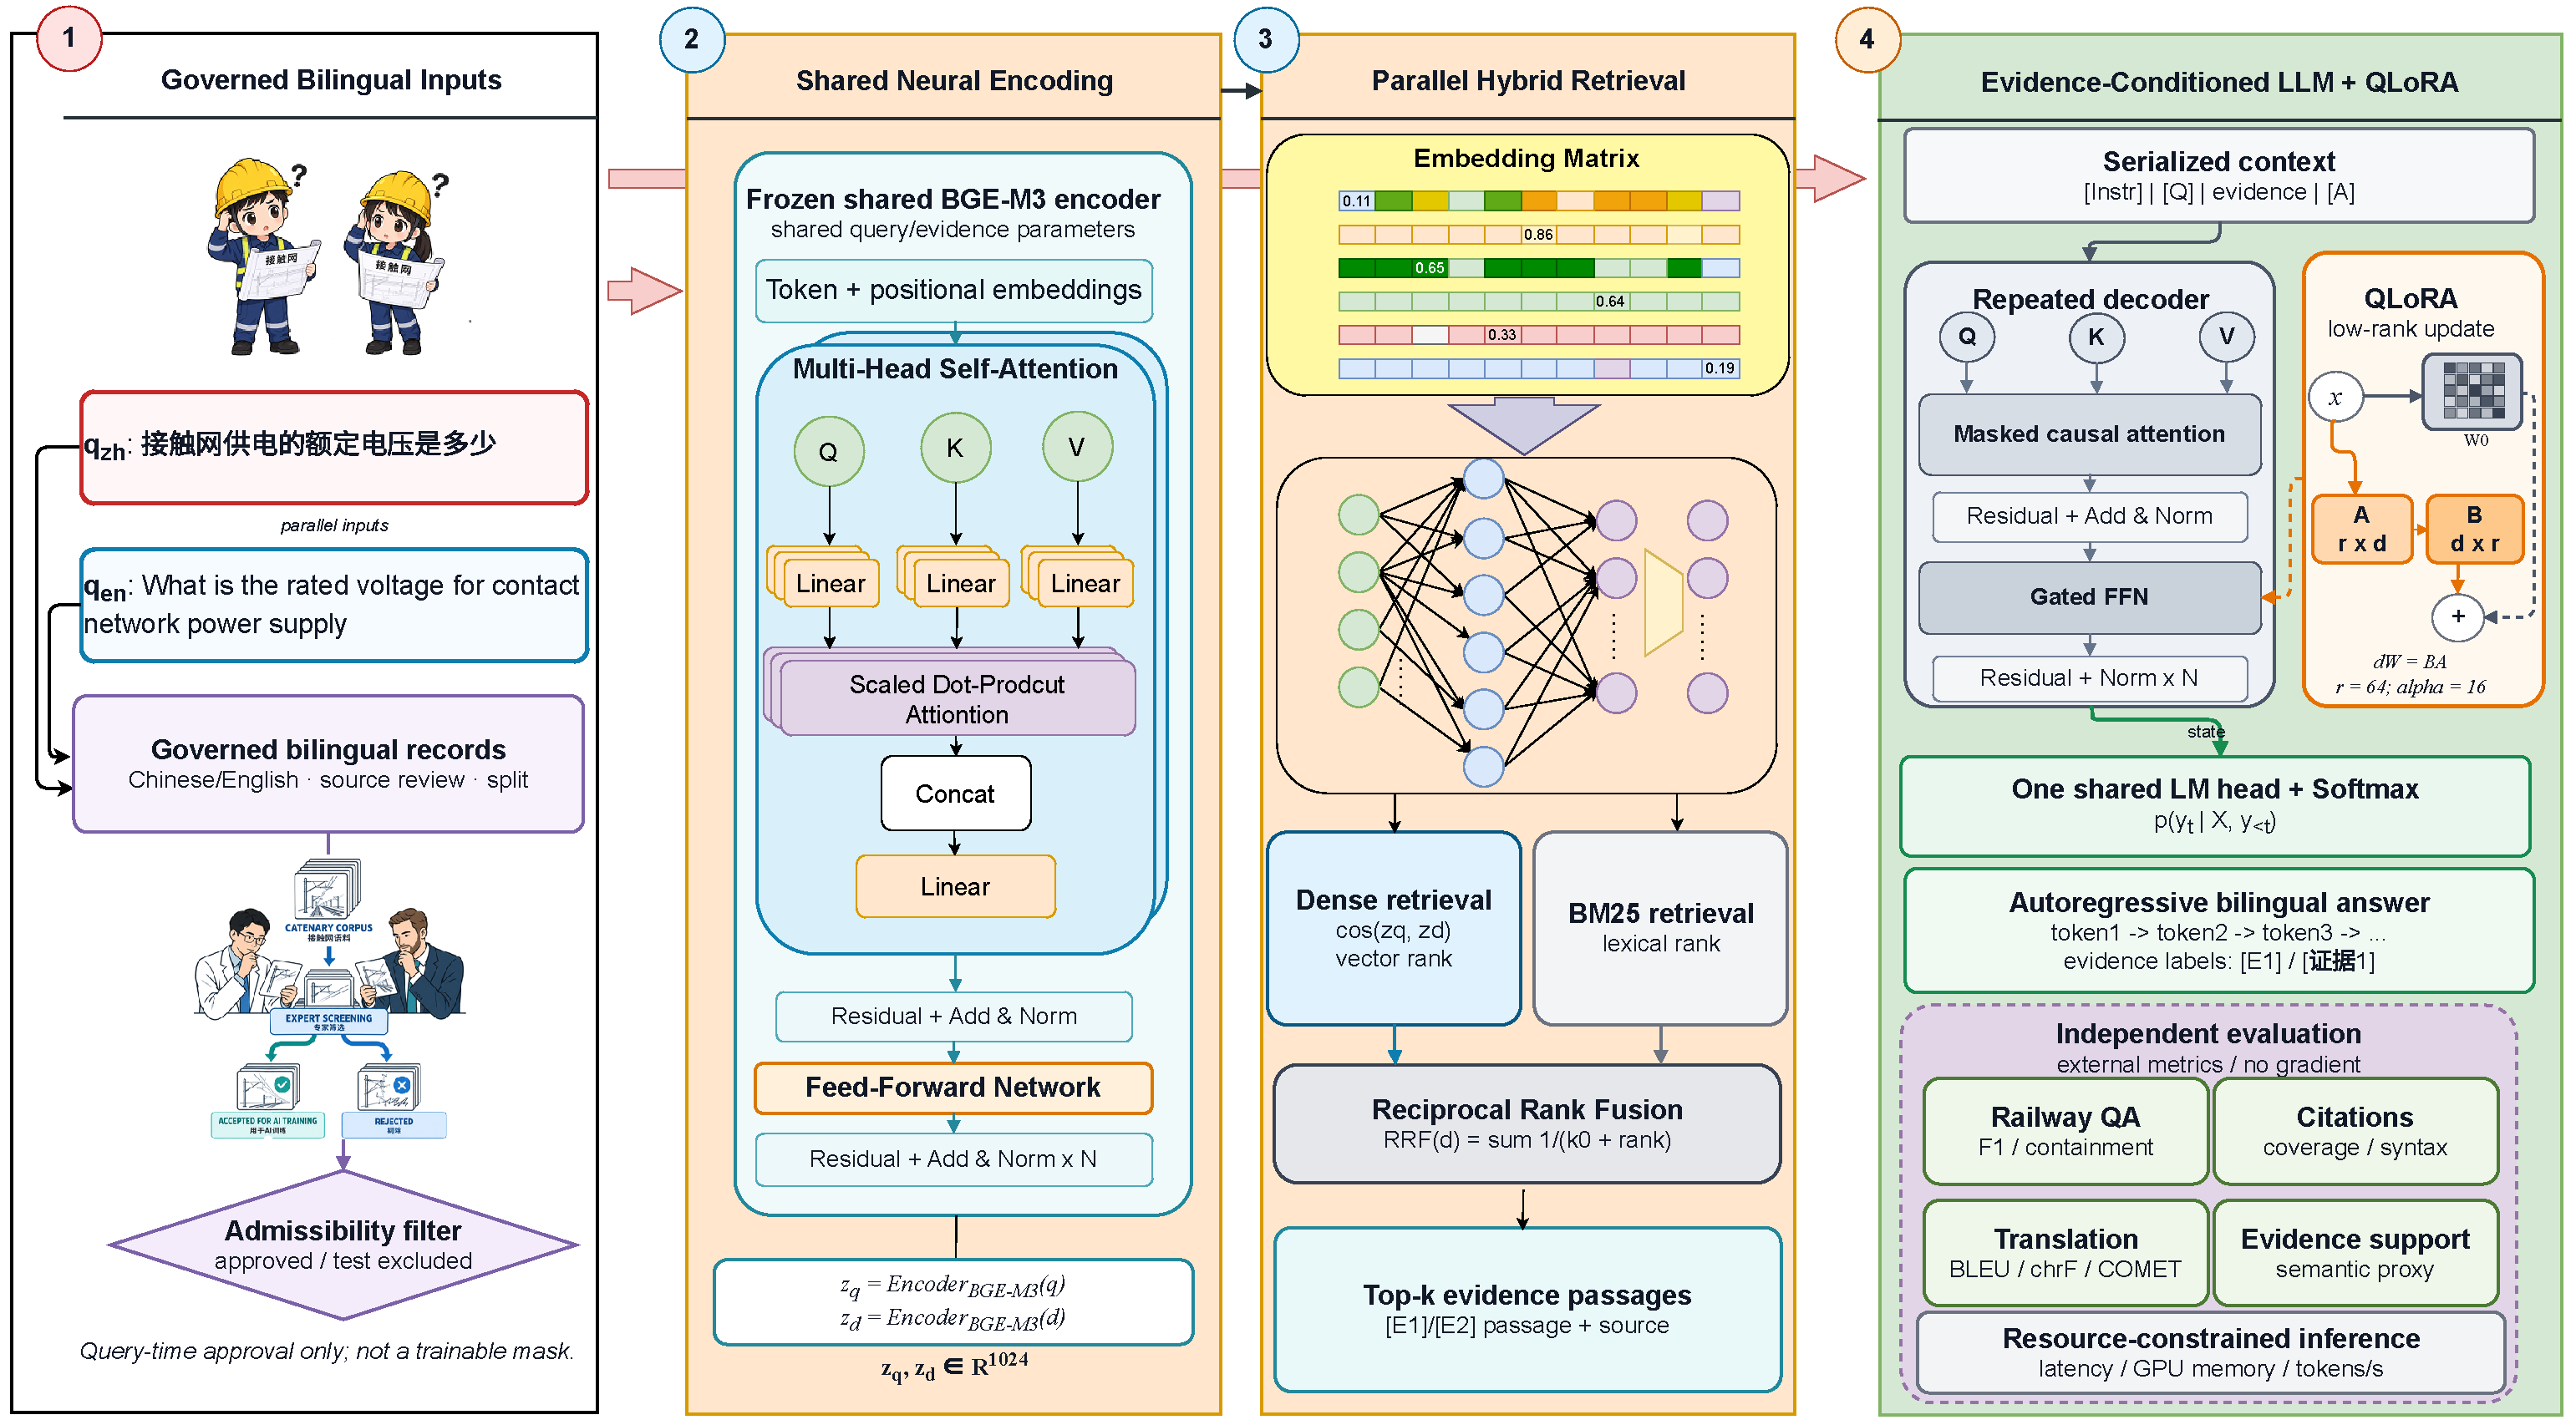
\includegraphics[width=0.92\linewidth,height=0.78\textheight,keepaspectratio]{figures/figure_01_neural_retrieval.pdf}
\caption{Knowledge-enhanced adaptation of the railway domain LLM. The evidence path combines BM25 lexical ranking and BGE-M3 dense ranking through reciprocal rank fusion before adding top-ranked railway passages to the prompt. The adaptation path trains completion-only QLoRA parameters while keeping the base model frozen. The two paths are evaluated separately and jointly to distinguish retrieval gains, domain-adaptation gains and their resource cost.}
\label{fig:neural-retrieval-qlora}
\end{figure}

\subsection{Hybrid retrieval and evidence-conditioned generation}

BM25 indexes Chinese and English question-answer fields and evidence, preserving exact matches for railway terms, equipment names and regulation identifiers. Dense search embeds the query with BGE-M3 and ranks semantically related passages by vector similarity. Reciprocal rank fusion combines the two rankings, and the approved-only condition excludes ineligible or held-out records before ranking. The top-ranked passages are numbered and inserted into the model prompt, enabling the generator to answer in the query language with explicit evidence labels.

Following Cormack \emph{et al.} (2009), the reciprocal-rank-fusion score for a candidate document \emph{d} is defined in Equation (1):

\begin{equation}
\operatorname{RRF}(d)=\sum_{r \in \{\mathrm{BM25},\mathrm{vector}\}}\frac{1}{k_0+\operatorname{rank}_r(d)}.
\end{equation}

In Equation (1), a document absent from a retriever's candidate list contributes zero for that retriever. The candidate pool is fixed at 50 per retriever and the conventional rank constant is $k_0=60$; Equation (1) is applied before final top-\emph{k} is varied. This controlled top-\emph{k} comparison changes the amount of evidence delivered to the generator without changing the upstream search pool. Every returned evidence object contains its record identifier, source document, task type and retrieval score.

For query and candidate embeddings, dense retrieval uses cosine similarity:

\begin{equation}
s_{\mathrm{dense}}(q,d)=\frac{\mathbf{e}_q^{\top}\mathbf{e}_d}{\lVert\mathbf{e}_q\rVert_2\lVert\mathbf{e}_d\rVert_2}.
\end{equation}

The completion-only adaptation objective is computed on answer positions only. If $m_t$ is one for an answer token and zero for a masked prompt token, the optimisation target is:

\begin{equation}
\mathcal{L}_{\mathrm{answer}}(\theta_A)=-\frac{1}{\sum_t m_t}\sum_t m_t\log p_{\theta_0,\theta_A}(y_t\mid y_{<t},x).
\end{equation}

Here $\theta_0$ denotes frozen NF4 base weights and $\theta_A$ denotes trainable LoRA parameters. For an answer prediction $\hat{y}$ and reference $y$, the character-level overlap used for standalone bilingual QA is:

\begin{equation}
P=\frac{|\hat{y}\cap y|}{|\hat{y}|},\qquad R=\frac{|\hat{y}\cap y|}{|y|},\qquad F1=\frac{2PR}{P+R}.
\end{equation}

The trained model and retriever are exposed through a local Vite and FastAPI interface for testing, but interface design is outside the experimental comparison. The reported results concern evidence retrieval, model outputs and resource use. Answers are described as evidence-conditioned because retrieved passages are included in the prompt; citation-format compliance and semantic support are evaluated separately.

\subsection{Resource-constrained QLoRA domain adaptation}

The adaptation dataset is generated only from approved records and split by knowledge-pair identifier, task type and source document. Chinese and English variants of the same knowledge item are assigned to the same partition. The current frozen 80/10/10 corpus contains 12,178 training, 1,524 validation and 1,526 test examples, balanced equally by language, with zero knowledge-pair identifier overlap among partitions. The 120 regulation items reserved for RAG evaluation are forced into the test partition and never used for training. Loss is computed only on answer tokens; all prompt labels are masked with Minus 100.

Qwen2.5-7B-Instruct and GLM-4-9B-Chat-HF form the adaptation matrix; their architectures and post-training lineage are documented in the corresponding official technical reports \citep{qwen2024technical,glm2024chatglm}. Both were loaded with NF4 quantisation and PEFT adapters on the target GPU. Qwen exposes separate Gate Projection and Up Projection modules, whereas GLM uses a fused Gate-Up Projection, requiring model-specific target lists. The Rank-64 configuration trained 161,480,704 Qwen parameters and 190,382,080 GLM parameters, representing 3.58 and 3.45 per cent of the parameters visible to the quantised training process, respectively. Qwen3-14B is retained as an unadapted larger reference generator \citep{qwen2025technical}.

Both runs use LoRA Rank 64, Alpha 16, Dropout 0.05, Learning Rate 2e-4, Maximum Sequence Length 1,024 and one epoch. The Per-Device Batch Size is one with 16 Gradient Accumulation Steps and a 0.03 Warm-Up Ratio. Random Seed 42 is fixed in the experiment configuration. Generation uses greedy decoding with Temperature 0 and Top-P 1, plus a task-dependent output limit. Completion-only supervision masks every prompt token with label minus 100, so training optimises the railway answer sequence rather than reproducing instructions.

\subsection{Evaluation design}

Retrieval conditions are BM25, vector, hybrid and approved hybrid. Metrics are evidence-equivalent Recall@1/3/5, MRR and mean latency. The formal generator matrix fixes no retrieval, BM25-RAG and approved hybrid-RAG so that five generators receive identical cached contexts. Automatic metrics include Answer F1, reference containment, citation-format coverage, citation omission and end-to-end latency. Citation measures are instruction-following indicators, not evidence-entailment or factual-hallucination measures. A supplementary directional translation check is retained only as a diagnostic and does not define the primary model outcome. The separate metrics prevent a retrieval score, answer score or resource measure from standing in for the other outcomes \citep{chang2024survey}.

Evidence-equivalent Recall@\emph{k} is one when at least one of the first \emph{k} candidates satisfies the frozen matching rule: the same record identifier, normalised gold and candidate evidence containment in either direction, or the same source document with the gold answer contained in candidate evidence. Because exact RAG-test records are excluded from the production index, observed hits normally arise from the latter evidence-equivalence criteria rather than identity. MRR averages the reciprocal rank of the first such match. The standalone bilingual QA evaluation uses character-level F1 in both languages: precision and recall are computed from multiset character overlap after answer normalisation and whitespace removal. The paired QA tests use this same metric. The RAG evaluation instead computes overlap F1 over individual Chinese characters and lower-cased Latin/alphanumeric word tokens. These two F1 definitions are reported within their respective evaluation settings, not treated as interchangeable absolute scores. In standalone QA, reference containment is a binary indicator of whether the normalised reference occurs in the prediction. In RAG, the stored reference-containment score is one when the whitespace-normalised reference is contained in the prediction, otherwise it falls back to RAG F1; empty predictions or references score zero. This is a graded containment score, not a binary containment rate. Citation-format coverage records only whether the requested evidence-label syntax appears; its complement is reported as citation omission.

All core comparisons use paired samples. Mean metrics are accompanied by 2,000-resample bootstrap 95 per cent confidence intervals in the released analysis tables. Original-versus-QLoRA comparisons use two-sided paired Wilcoxon tests, Cohen's \emph{d}\textsubscript{z} for paired effects and Holm correction across the pre-specified family recorded in the analysis configuration. Exploratory error categories are reported separately and are not treated as confirmatory hypothesis tests. Efficiency measurements use 30 Chinese short questions, 30 English short questions and 30 regulation-oriented long-context questions, with one warm-up and three measured repetitions per model condition.

\subsection{Resource-constrained implementation}

Table I defines the single-workstation boundary used throughout the experiments. The adapted 7B and 9B models require neither multi-GPU training nor cloud inference, allowing retrieval, adaptation and generation to be tested on hardware available to a small institutional laboratory.

\begin{table}[ht]
\centering
\caption{Single-workstation implementation and experimental configuration.}

\begin{tabular}{p{0.28\linewidth}p{0.64\linewidth}}
\toprule
Component & Formal setting \\
\midrule
Database & PostgreSQL 16.14; pgvector 0.8.4 \\
Embedding & BAAI/bge-m3; 1,024 dimensions \\
Adapted generators & Qwen2.5-7B-Instruct; GLM-4-9B-Chat-HF \\
Reference generator & Qwen3-14B through Ollama 0.19.0 \\
Training & NF4 QLoRA; rank 64; one epoch; seed 42 \\
Hardware boundary & One RTX 3090 24 GB; 32 GB RAM; no multi-GPU or required cloud inference \\
Statistical analysis & 2,000 bootstrap resamples; paired Wilcoxon; Cohen's \emph{d}\textsubscript{z}; Holm correction \\
Software & Linux; Python 3.11.15; PyTorch 2.11.0; Transformers 5.12.1; PEFT 0.18.1; bitsandbytes 0.49.2; Ollama 0.19.0 \\
\bottomrule
\end{tabular}
\end{table}

The code separates test-set construction, embedding, retrieval evaluation, generator evaluation, adaptation and report export. This prevents an analysis script from silently changing the production index or training split. Cached retrieval contexts are reused across generators in the formal RAG matrix, so model comparisons receive identical evidence. The manifest records the Git state and every input hash at freeze time, supporting result reconstruction and consistent comparison across runs.

Production embedding loading is local-files-only by default. The environment, model revisions, split statistics and asset hashes are recorded with the comparison outputs so that the reported resource boundary can be reconstructed.

\section{Results}

\subsection{Knowledge-base composition}

The database contains 37,661 approved records and 37,109 complete bilingual records. After freezing the formal RAG test, 37,261 approved non-test knowledge chunks have BGE-M3 embeddings. The QLoRA test partition contains 763 knowledge pairs across four source documents. From this partition, the formal cross-source RAG set contains 400 knowledge pairs and 800 language-specific queries: 150 regulation, 127 terminology and 123 textbook/concept pairs across 17 task types. The earlier 120-pair regulation pilot is a subset of this formal set and remains available in the reproducibility artifacts; it is not reported as an additional sample in the main results.

\subsection{Formal cross-source bilingual retrieval}

\begin{table}[ht]
\centering
\caption{Formal cross-source evidence-equivalent retrieval on 400 knowledge pairs.}

\small
\begin{adjustbox}{max width=\linewidth}
\begin{tabular}{>{\raggedright\arraybackslash}p{0.19\linewidth}lrrrrr}
\toprule
Retrieval & Language & Evidence R@1 & Evidence R@3 & Evidence R@5 & MRR & Mean latency (ms) \\
\midrule
BM25 & Chinese & 0.520 & 0.595 & 0.620 & 0.560 & \textbf{69.5} \\
Vector & Chinese & 0.518 & 0.653 & 0.690 & 0.588 & 134.4 \\
Hybrid approved & Chinese & \textbf{0.570} & \textbf{0.675} & \textbf{0.715} & \textbf{0.628} & 217.6 \\
BM25 & English & \textbf{0.570} & \textbf{0.670} & 0.685 & 0.620 & \textbf{59.0} \\
Vector & English & 0.463 & 0.553 & 0.580 & 0.509 & 134.4 \\
Hybrid approved & English & \textbf{0.570} & 0.668 & \textbf{0.708} & \textbf{0.620} & 209.2 \\
\bottomrule
\end{tabular}
\end{adjustbox}
\end{table}

Table II reports the formal evidence-equivalent retrieval comparison. BM25 is particularly competitive for English terminology queries, while dense retrieval records higher Chinese evidence recall in this evaluation. Hybrid fusion combines these strengths and obtains the highest Evidence Recall@5 in both languages: 0.715 in Chinese and 0.708 in English. Its mean latency is approximately three times that of BM25, so the gain is a quality--latency trade-off rather than a universal efficiency advantage. Approved-only and unfiltered hybrid results are identical because all admissible indexed records in this frozen experiment satisfy the approval condition.


\begin{figure}[ht]
\centering
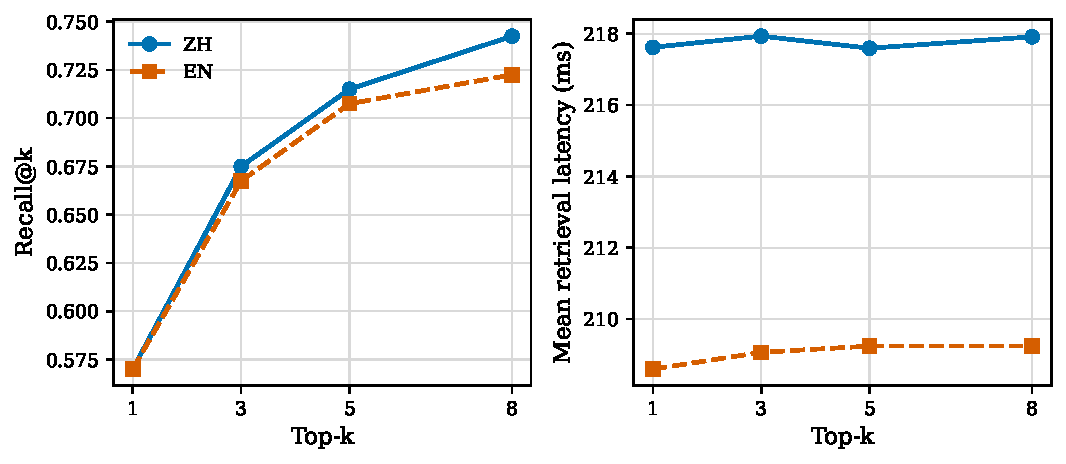
\includegraphics[width=0.82\linewidth,keepaspectratio]{figures/figure_03_top_k_quality_latency.pdf}
\caption{Effect of the final evidence cutoff on hybrid retrieval. Recall rises from 0.570 at top-1 to 0.743/0.723 at top-8 for Chinese/English, whereas mean retrieval latency remains near 218/209 ms because the upstream candidate pool is fixed. The figure shows that returning more fused candidates improves evidence coverage without materially changing search time in this experiment. Source: Authors' own work.}
\end{figure}

Figure 2 shows a consistent recall gain as the final cutoff increases from one to eight. The largest gain occurs between top-1 and top-3, followed by smaller improvements at top-5 and top-8. In contrast, the latency curves remain nearly flat because each setting reuses the same 50-candidate BM25 and dense search pools. The objective advantage is therefore greater evidence coverage at a larger final cutoff without additional upstream retrieval work; the generator may still incur extra context cost when more passages are supplied.

\subsection{QLoRA adaptation and held-out QA}

Having established the retrieval results, the next analysis examines the effect of QLoRA adaptation on held-out question answering.

Figure 3 presents the completion-only QLoRA training trajectories. Both models show a steep initial reduction followed by a slower decline, and their end-of-epoch validation losses remain close to the final training region. Qwen finishes with lower training and validation loss than GLM, which is consistent with its stronger held-out bilingual QA result. The figure supports successful one-epoch optimisation under the resource limit, but it does not establish convergence across longer schedules or repeated random seeds.

On the 1,526-example held-out bilingual QA set, Qwen QLoRA increased character-level F1 from 0.189 (95 per cent CI 0.175-0.204) to 0.398 (0.376-0.422) in Chinese and from 0.437 (0.419-0.455) to 0.648 (0.632-0.664) in English. GLM increased from 0.192 to 0.410 in Chinese and from 0.498 to 0.552 in English. All four paired gains remained significant after Holm correction (all adjusted p-values below 0.01); Cohen's \emph{d}\textsubscript{z} was 0.569 and 0.634 for Qwen Chinese and English, and 0.614 and 0.146 for GLM. Qwen provides the strongest balanced adapted QA result under this character-level metric; the small GLM English effect cautions against pooling languages. These sample-level tests do not estimate variation across repeated training seeds.

\begin{figure}[ht]
\centering
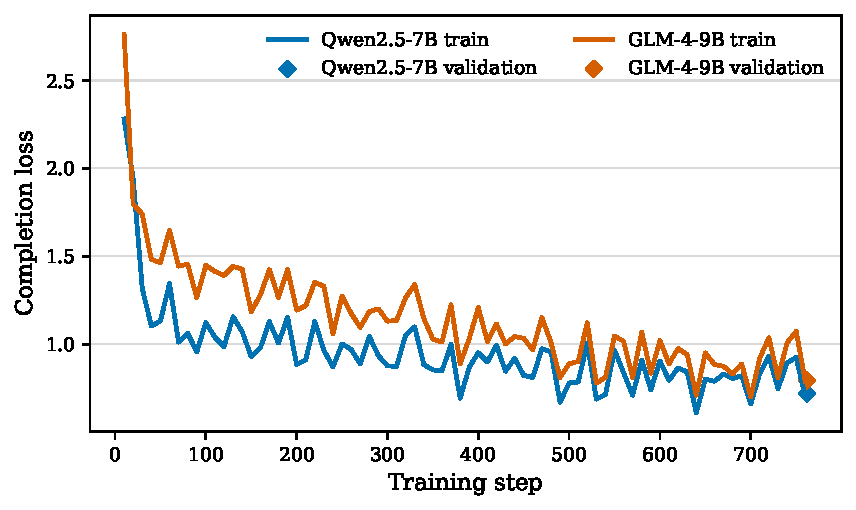
\includegraphics[width=0.82\linewidth,keepaspectratio]{figures/figure_04_training_validation_loss.pdf}
\caption{One-epoch completion-only QLoRA optimisation. Training loss declines rapidly for both models and then stabilises, while the end-of-epoch validation diamonds remain near the final training-loss range. Qwen ends below GLM on both curves, providing optimisation evidence consistent with its stronger held-out QA score. Source: Authors' own work.}
\end{figure}

\subsection{Multi-generator RAG comparisons}

The held-out QA results motivate the next comparison, which tests how retrieved evidence changes answer quality across generators.

Approved-hybrid RAG significantly improved Answer F1 over no retrieval for every generator and language after Holm correction. Table III summarises the main comparisons; the adjusted p-values are below 0.01 in every language-model condition. The results show that Qwen QLoRA achieved the highest absolute hybrid-RAG F1, whereas original Qwen obtained the largest incremental gain from adding retrieval. BM25 and hybrid did not have a uniform answer-quality ordering, so the observed gains depend on adaptation, retrieval strategy and language.

\begin{table}[ht]
\centering
\caption{Multi-generator RAG comparison.}

\small
\begin{adjustbox}{max width=\linewidth}
\begin{tabular}{>{\raggedright\arraybackslash}p{0.18\linewidth}p{0.19\linewidth}p{0.19\linewidth}p{0.18\linewidth}p{0.20\linewidth}}
\toprule
Generator & No retrieval F1 (ZH/EN) & Approved-hybrid F1 (ZH/EN) & Gain (ZH/EN) & Holm-adjusted \emph{p} (ZH/EN) \\
\midrule
Original Qwen & 0.262 / 0.306 & 0.402 / 0.440 & +0.141 / +0.133 & 1.89e-39 / 2.28e-42 \\
Original GLM & 0.230 / 0.269 & 0.297 / 0.318 & +0.067 / +0.048 & 1.13e-22 / 9.56e-31 \\
Qwen QLoRA & 0.630 / 0.573 & 0.660 / 0.651 & +0.030 / +0.078 & 1.34e-06 / 1.41e-11 \\
GLM QLoRA & 0.398 / 0.331 & 0.476 / 0.351 & +0.077 / +0.020 & 3.16e-09 / 9.37e-03 \\
Qwen3-14B & 0.295 / 0.336 & 0.442 / 0.454 & +0.147 / +0.118 & 6.66e-32 / 7.58e-29 \\
\bottomrule
\end{tabular}
\end{adjustbox}
\end{table}

Here, each cell reports Chinese/English values; no value is omitted in the comparison. The paired significance values correspond to the no-retrieval versus approved-hybrid comparison.

The traceability result was different. For original Qwen, citation-format coverage moved from 0.543/0.638 under BM25 to 0.595/0.643 under hybrid in Chinese/English; Qwen3 moved from 0.715/0.900 to 0.788/0.905. By contrast, Qwen QLoRA achieved only 0.000/0.003 under hybrid, and GLM showed the same, less extreme adaptation-related pattern. In the tested conditions, QLoRA produced stronger answer overlap but weaker compliance with the citation instruction used in the evaluation targets; citation omission approached one for the adapted models. This is an instruction-following failure, not a measured factual hallucination rate. For railway-domain answering, Qwen2.5 QLoRA provides the strongest answer overlap, while original Qwen and Qwen3 show stronger citation-format compliance until citation-aware adaptation is added.

\subsection{Supplementary translation check}

A supplementary translation check produced direction- and task-dependent changes after adaptation. Because the primary objective is railway-domain question answering, these translation results are retained only as a diagnostic and are not used to define the main model improvement.


\begin{figure}[ht]
\centering

\includegraphics[width=0.82\linewidth,keepaspectratio]{figures/figure_06_quality_latency_pareto.pdf}
\caption{Quality--resource comparison for original and QLoRA-adapted models. Qwen QLoRA has the highest mean bilingual QA F1, while remaining within the 24 GB GPU limit; its higher latency and reserved memory show the cost of this gain. The low latency of GLM QLoRA reflects abnormally short or empty outputs and is not interpreted as an efficiency advantage. Source: Authors' own work.}
\end{figure}

\subsection{Resource use}

Resource measurements test whether the domain-adapted models remain executable on the defined single workstation and show the cost associated with their QA gains.

All five deployment conditions completed 270 measurements without execution failure or OOM. GPU memory measurements are expressed in GiB (2\textasciicircum{}30 bytes). Original Qwen and GLM reached 5.49 and 6.76 GiB peak PyTorch reserved memory and generated at 31.9 and 22.7 tokens/s. Their QLoRA variants reached 16.11 and 19.49 GiB and generated at 17.5 and 11.9 tokens/s. Peak allocated memory was 5.35 and 6.48 GiB for the original models, compared with 15.40 and 7.20 GiB for the QLoRA variants. Reserved memory includes caching-allocator reservations and should not be interpreted as memory occupied by live tensors or as the intrinsic adapter overhead. Qwen3-14B through Ollama reached 14.26 GiB of GPU-process memory and 78.5 tokens/s; this memory statistic is not PyTorch reserved memory, and cross-backend memory and timing comparisons are descriptive. The Qwen and GLM adapters occupy approximately 627 and 746 MB. The low 2.63 s GLM QLoRA mean latency reflects abnormally short or empty outputs and is not an efficiency advantage. All configurations fit the target 24 GB workstation, but original Qwen provides the lowest resource cost and Qwen QLoRA the strongest QA quality within the limit.

Figure 4 relates mean bilingual standalone QA F1 to generation latency and peak reserved GPU memory. Qwen QLoRA occupies the highest-quality position in both panels and remains below the 24 GB boundary, demonstrating that the strongest adapted QA result is attainable on the target workstation. The original models use substantially less memory, so adaptation improves quality at a measurable resource cost. The plot is descriptive rather than a controlled causal estimate of adapter overhead, and Qwen3 through Ollama is excluded because its backend reports a different memory statistic.


\subsection{Supplementary evidence and corpus-control checks}

Figure 5 examines whether the knowledge component behind the domain model behaves as intended. It compares language-field choices, checks whether generated claims are supported by retrieved or explicitly cited evidence, and records corpus review operations. These checks supplement the primary retrieval and QA results.

\begin{figure}[H]
\centering

\includegraphics[width=0.82\linewidth,keepaspectratio]{figures/figure_08_system_validation.pdf}
\caption{Supplementary validation of the knowledge-enhanced model. Panel A shows that the bilingual index provides the strongest cross-language Recall@5 balance. Panel B shows high semantic support from retrieved evidence but substantially lower support through explicit citations, especially after QLoRA. Panel C confirms that corpus approval and edit operations are recorded. The panels distinguish evidence access, visible attribution and data control rather than combining them into one quality claim.}
\end{figure}

\begin{table}[H]
\centering
\caption{Supplementary evidence-access, attribution and corpus-control results.}

\begin{adjustbox}{max width=\linewidth}
\begin{tabular}{llll}
\toprule
Validation & Chinese & English & Operational result \\
\midrule
Bilingual-field hybrid index, Evidence Recall@5 & 0.718 & 0.675 & Highest balanced mean (0.696) \\
Original Qwen hybrid, supported-claim proxy & 0.878 & 0.836 & Citation precision 0.955/0.970 \\
Qwen QLoRA hybrid, supported-claim proxy & 0.964 & 0.905 & Citation recall 0.000/0.002 \\
Governance history & — & — & 1,337 events; 82 edits; two recorded reviewers \\
\bottomrule
\end{tabular}
\end{adjustbox}
\end{table}

Panel A of Figure 5 shows why bilingual indexing is retained: it reaches 0.718 Recall@5 in Chinese and 0.675 in English, giving the highest balanced mean of 0.696, although the English-only field remains better on English alone. Panel B shows that the generated claims generally have strong semantic support somewhere in the retrieved context, including 0.964/0.905 for Qwen QLoRA in Chinese/English. The much lower explicitly cited support reveals a separate attribution weakness; retrieval can provide useful evidence even when the adapted model does not reproduce the requested citation labels. Panel C records 1,337 corpus operations and the fields changed during edits, confirming that the evidence used for training and retrieval has an inspectable history. The figure therefore demonstrates the advantage of bilingual evidence access while also locating the remaining weakness in citation behaviour rather than in retrieval support itself.

\clearpage

\section{Discussion}

\subsection{Effectiveness of hybrid evidence retrieval}

The retrieval experiments show that lexical and dense signals solve different parts of the railway evidence problem. BM25 remains strong for exact English terminology and regulation identifiers, while BGE-M3 retrieves more semantically related Chinese evidence. Reciprocal rank fusion preserves useful candidates from both rankings and produces the highest Evidence Recall@5 in Chinese and English. The bilingual-field ablation adds a second result: indexing both language fields gives the strongest balance across languages, even though a language-specific index can lead on one language alone. These findings support hybrid retrieval as the knowledge-access component of the railway domain LLM \citep{robertson2009bm25,cormack2009rrf}.

The gain is not cost-free. Hybrid search takes approximately three times the latency of BM25, and increasing the number of passages can enlarge the generator context. However, Figure 2 shows that changing the final cutoff from top-1 to top-8 raises evidence recall while leaving retrieval latency nearly constant under the fixed candidate pool. This gives a practical control for choosing evidence coverage according to the available context budget.

\subsection{Effectiveness of low-resource domain adaptation}

Completion-only QLoRA improves held-out railway QA for both model families and both languages. The gains are strongest and most balanced for Qwen2.5-7B, which also reaches the highest Answer F1 after hybrid evidence is added. The generator matrix further shows that approved-hybrid RAG improves Answer F1 over no retrieval for every evaluated model and language. Retrieved knowledge and parameter adaptation therefore provide distinct benefits: retrieval improves every generator, while QLoRA gives the medium-sized Qwen model the strongest absolute railway QA result.

This distinction matters for vertical-domain modelling. A larger unadapted reference model does not replace either railway evidence access or target-domain adaptation. Conversely, adaptation alone does not guarantee correct evidence attribution. Qwen QLoRA retains high semantic support against retrieved passages but weak citation-label coverage, indicating that answer quality and visible attribution require different optimisation targets.

\subsection{Resource--quality trade-off and limitations}

All evaluated models run within the 24 GB GPU boundary, confirming that the approach is feasible without multi-GPU training. Figure 4 nevertheless shows a clear trade-off: Qwen QLoRA provides the strongest QA quality but uses more reserved memory and generation time than the original model. GLM QLoRA also consumes more memory, and its abnormally short outputs mean that low measured latency cannot be interpreted as useful efficiency. The evidence supports local feasibility, not negligible adaptation cost.

The study is limited to one frozen corpus split, one epoch and one principal random seed. The sample-level significance tests do not measure variation across repeated training runs, and evidence-equivalent recall depends on the predefined matching rule. Citation-format compliance is also weaker for adapted models. These boundaries limit broad claims while leaving the main finding intact: under the tested resource constraint, hybrid evidence retrieval and QLoRA jointly improve railway-domain question answering.

\section{Conclusion}

This study develops a knowledge-enhanced railway domain LLM for bilingual vocational education under a single-workstation resource constraint. BM25 and BGE-M3 provide complementary rankings, and reciprocal rank fusion achieves the strongest Evidence Recall@5 in both languages. Completion-only QLoRA substantially improves held-out railway QA, with Qwen2.5-7B producing the strongest balanced adapted result. When hybrid evidence is added, Answer F1 improves for every evaluated generator and language. These results show that a medium-sized model can gain both domain knowledge access and domain-specific answering ability without multi-GPU training. The remaining citation and repeated-run limitations identify where evaluation and adaptation should be strengthened, but they do not alter the observed retrieval and railway QA gains.

\bibliographystyle{apalike}
\begin{thebibliography}{}

\bibitem[Barnett et~al., 2024]{barnett2024finetuning}
Barnett, S., Brannelly, Z., Kurniawan, S., and Wong, S. (2024).
\newblock Fine-tuning or fine-failing? debunking performance myths in large
  language models.
\newblock {\em arXiv preprint arXiv:2406.11201}.
\newblock Available at: \url{https://arxiv.org/abs/2406.11201}.

\bibitem[Chang et~al., 2024]{chang2024survey}
Chang, Y., Wang, X., Wang, J., Wu, Y., Yang, L., Zhu, K., Chen, H., Yi, X.,
  Wang, C., Wang, Y., Ye, W., Zhang, Y., Chang, Y., Yu, P.~S., Yang, Q., and
  Xie, X. (2024).
\newblock A survey on evaluation of large language models.
\newblock {\em ACM Transactions on Intelligent Systems and Technology},
  15(3):1--45.
\newblock DOI: \url{https://doi.org/10.1145/3641289}.

\bibitem[Chen et~al., 2024]{chen2024bgem3}
Chen, J., Xiao, S., Zhang, P., Luo, K., Lian, D., and Liu, Z. (2024).
\newblock Bge m3-embedding: Multi-lingual, multi-functionality,
  multi-granularity text embeddings through self-knowledge distillation.
\newblock {\em arXiv preprint arXiv:2402.03216}.
\newblock Available at: \url{https://arxiv.org/abs/2402.03216}.

\bibitem[Cormack et~al., 2009]{cormack2009rrf}
Cormack, G.~V., Clarke, C. L.~A., and Buettcher, S. (2009).
\newblock Reciprocal rank fusion outperforms condorcet and individual rank
  learning methods.
\newblock In {\em Proceedings of the 32nd International ACM SIGIR Conference},
  pages 758--759.
\newblock DOI: \url{https://doi.org/10.1145/1571941.1572114}.

\bibitem[Dettmers et~al., 2023]{dettmers2023qlora}
Dettmers, T., Pagnoni, A., Holtzman, A., and Zettlemoyer, L. (2023).
\newblock Qlora: Efficient finetuning of quantized llms.
\newblock In {\em Advances in Neural Information Processing Systems},
  volume~36.
\newblock Available at: \url{https://arxiv.org/abs/2305.14314}.

\bibitem[Ding et~al., 2023]{ding2023peft}
Ding, N., Qin, Y., Yang, G., Wei, F., Yang, Z., Su, Y., Hu, S., Chen, Y., Chan,
  C.-M., and Chen, W. (2023).
\newblock Parameter-efficient fine-tuning of large-scale pre-trained language
  models.
\newblock {\em Nature Machine Intelligence}, 5(3):220--235.
\newblock DOI: \url{https://doi.org/10.1038/s42256-023-00626-4}.

\bibitem[{GLM Team}, 2024]{glm2024chatglm}
{GLM Team} (2024).
\newblock Chatglm: a family of large language models from glm-130b to glm-4 all
  tools.
\newblock Available at: \url{https://arxiv.org/abs/2406.12793}.

\bibitem[Huang et~al., 2026]{huang2026emergency}
Huang, L., Liu, Z., Yu, C., Zhu, T., and Yan, B. (2026).
\newblock Emergency operation scheme generation for urban rail transit train
  door systems using retrieval-augmented large language models.
\newblock {\em Sensors}, 26(6):2006.
\newblock DOI: \url{https://doi.org/10.3390/s26062006}.

\bibitem[H{\"u}bscher et~al., 2021]{hubscher2021knowledge}
H{\"u}bscher, G., Geist, V., Auer, D., H{\"u}bscher, N., and K{\"u}ng, J.
  (2021).
\newblock Representation and presentation of knowledge and processes -- an
  integrated approach for a dynamic communication-intensive environment.
\newblock {\em International Journal of Web Information Systems},
  17(6):669--697.
\newblock DOI: \url{https://doi.org/10.1108/IJWIS-03-2021-0031}.

\bibitem[Kasneci et~al., 2023]{kasneci2023chatgpt}
Kasneci, E., Sessler, K., K{\"u}chemann, S., Bannert, M., Dementieva, D.,
  Fischer, F., Gasser, U., Groh, G., G{\"u}nnemann, S., H{\"u}llermeier, E.,
  Krusche, S., Kutyniok, G., Michaeli, T., Nerdel, C., Pfeffer, J., Poquet, O.,
  Sailer, M., Schmidt, A., Seidel, T., Stadler, M., Weller, J., Kuhn, J., and
  Kasneci, G. (2023).
\newblock Chatgpt for good? on opportunities and challenges of large language
  models for education.
\newblock {\em Learning and Individual Differences}, 103:102274.
\newblock DOI: \url{https://doi.org/10.1016/j.lindif.2023.102274}.

\bibitem[Lahnalampi, 2024]{lahnalampi2024rail}
Lahnalampi, A. (2024).
\newblock Utilizing large language models in rail design projects.
\newblock Master's thesis, Aalto University.
\newblock Available at:
  \url{https://aaltodoc.aalto.fi/items/87b7ac34-756c-4db2-8bea-f9b9e6b453ed}.

\bibitem[Lawrence et~al., 2019]{lawrence2019hsr}
Lawrence, M., Bullock, R., and Liu, Z. (2019).
\newblock {\em China's High-Speed Rail Development}.
\newblock World Bank, Washington, DC.
\newblock DOI: \url{https://doi.org/10.1596/978-1-4648-1425-9}.

\bibitem[Lewis et~al., 2020]{lewis2020rag}
Lewis, P., Perez, E., Piktus, A., Petroni, F., Karpukhin, V., Goyal, N.,
  K{\"u}ttler, H., Lewis, M., Yih, W.-T., Rockt{\"a}schel, T., Riedel, S., and
  Kiela, D. (2020).
\newblock Retrieval-augmented generation for knowledge-intensive nlp tasks.
\newblock In {\em Advances in Neural Information Processing Systems},
  volume~33, pages 9459--9474.
\newblock Available at: \url{https://arxiv.org/abs/2005.11401}.

\bibitem[Li et~al., 2024]{li2024rschat}
Li, J., Li, C., Niu, S., and Dai, B. (2024).
\newblock Rschat: intelligent question answering model for railway safety
  knowledge.
\newblock In {\em 2024 IEEE/ACIS 24th International Conference on Computer and
  Information Science}, pages 55--60.
\newblock DOI: \url{https://doi.org/10.1109/ICIS61260.2024.10778327}.

\bibitem[Li et~al., 2025]{li2025training}
Li, Y., Chen, J., Luo, X., and Zheng, H. (2025).
\newblock Intelligent human-computer interactive training assistant system for
  rail systems.
\newblock {\em High-speed Railway}, 3(1):64--77.
\newblock DOI: \url{https://doi.org/10.1016/j.hspr.2025.02.001}.

\bibitem[Luo et~al., 2025]{luo2025driver}
Luo, Y.~C., Xun, J., Wang, W., Zhang, R.~Z., and Zhao, Z.~C. (2025).
\newblock A driver advisory system based on large language model for high-speed
  train.
\newblock Available at: \url{https://arxiv.org/abs/2501.07837}.

\bibitem[Lv et~al., 2024]{lv2024full}
Lv, K., Yang, Y., Liu, T., Guo, Q., and Qiu, X. (2024).
\newblock Full parameter fine-tuning for large language models with limited
  resources.
\newblock In {\em Proceedings of the 62nd Annual Meeting of the Association for
  Computational Linguistics}, pages 8187--8198.
\newblock DOI: \url{https://doi.org/10.18653/v1/2024.acl-long.445}.

\bibitem[{Qwen Team}, 2024]{qwen2024technical}
{Qwen Team} (2024).
\newblock Qwen2.5 technical report.
\newblock Available at: \url{https://arxiv.org/abs/2412.15115}.

\bibitem[{Qwen Team}, 2025]{qwen2025technical}
{Qwen Team} (2025).
\newblock Qwen3 technical report.
\newblock Available at: \url{https://arxiv.org/abs/2505.09388}.

\bibitem[Robertson and Zaragoza, 2009]{robertson2009bm25}
Robertson, S. and Zaragoza, H. (2009).
\newblock The probabilistic relevance framework: Bm25 and beyond.
\newblock {\em Foundations and Trends in Information Retrieval}, 3(4):333--389.
\newblock DOI: \url{https://doi.org/10.1561/1500000019}.

\bibitem[Schwartz et~al., 2020]{schwartz2020green}
Schwartz, R., Dodge, J., Smith, N.~A., and Etzioni, O. (2020).
\newblock Green ai.
\newblock {\em Communications of the ACM}, 63(12):54--63.
\newblock DOI: \url{https://doi.org/10.1145/3381831}.

\bibitem[Song et~al., 2025]{song2025railway}
Song, Y., Tang, Y., and Liu, R. (2025).
\newblock Large language model and application for railway track management
  based on domain specialization.
\newblock In {\em The Proceedings of the 11th International Conference on
  Traffic and Transportation Studies}, volume 616, pages 194--204.
\newblock DOI: \url{https://doi.org/10.1007/978-981-97-9644-1_21}.

\bibitem[Tian et~al., 2024]{tian2024factuality}
Tian, K., Mitchell, E., Yao, H., Manning, C., and Finn, C. (2024).
\newblock Fine-tuning language models for factuality.
\newblock In {\em International Conference on Learning Representations}.
\newblock Available at:
  \url{https://proceedings.iclr.cc/paper_files/paper/2024/hash/c361ae924c23cafca6033610d25dbc65-Abstract-Conference.html}.

\bibitem[{UNESCO}, 2023]{unesco2023guidance}
{UNESCO} (2023).
\newblock Guidance for generative ai in education and research.
\newblock Available at:
  \url{https://unesdoc.unesco.org/ark:/48223/pf0000386693}.

\bibitem[Wandelt et~al., 2024]{wandelt2024transport}
Wandelt, S., Zheng, C., Wang, S., Liu, Y., and Sun, X. (2024).
\newblock Large language models for intelligent transportation: a review of the
  state of the art and challenges.
\newblock {\em Applied Sciences}, 14(17):7455.
\newblock DOI: \url{https://doi.org/10.3390/app14177455}.

\bibitem[Wang and Li, 2024]{wang2024phm}
Wang, H. and Li, Y.-F. (2024).
\newblock Large-scale language models for phm in railway systems: potential
  applications, limitations, and solutions.
\newblock In {\em Proceedings of the 6th International Conference on Electrical
  Engineering and Information Technologies for Rail Transportation}, volume
  1137, pages 591--599.
\newblock DOI: \url{https://doi.org/10.1007/978-981-99-9311-6_59}.

\bibitem[Wang et~al., 2025]{wang2025peft}
Wang, L., Chen, S., Jiang, L., Pan, S., Cai, R., Yang, S., and Yang, F. (2025).
\newblock Parameter-efficient fine-tuning in large language models: a survey of
  methodologies.
\newblock {\em Artificial Intelligence Review}, 58(8):227.
\newblock DOI: \url{https://doi.org/10.1007/s10462-025-11236-4}.

\bibitem[Xu, 2018]{xu2018education}
Xu, F. (2018).
\newblock Future of high-speed railway and university education.
\newblock In {\em The Belt and Road}, pages 167--183. Springer, Singapore.
\newblock DOI: \url{https://doi.org/10.1007/978-981-13-1105-5_7}.

\bibitem[Yang et~al., 2024]{yang2024legalqa}
Yang, X., Wang, Z., Wang, Q., Wei, K., Zhang, K., and Shi, J. (2024).
\newblock Large language models for automated q\&a involving legal documents: a
  survey on algorithms, frameworks and applications.
\newblock {\em International Journal of Web Information Systems},
  20(4):413--435.
\newblock DOI: \url{https://doi.org/10.1108/IJWIS-12-2023-0256}.

\bibitem[Zheng et~al., 2023]{zheng2023trafficsafety}
Zheng, O., Abdel-Aty, M., Wang, D., Wang, C., and Ding, S. (2023).
\newblock Trafficsafetygpt: tuning a pre-trained large language model to a
  domain-specific expert in transportation safety.
\newblock Available at: \url{https://arxiv.org/abs/2307.15311}.

\end{thebibliography}


\end{document}
